%\documentclass[final,1p,times,geometry={paperwidth=8.5in,paperheight=11in,margin=1in}]{elsarticle}
%\documentclass[12pt]{article}
\documentclass[final,1p,times]{elsarticle}
\geometry{reset,letterpaper,margin=1in}
\usepackage{amsmath,amssymb}
\usepackage{graphicx}
\usepackage{float}
\usepackage[T1]{fontenc}
\usepackage{ragged2e}
\usepackage{booktabs}
\usepackage{xcolor}
\usepackage{needspace}
\ifdefined\pdfmapfile\pdfmapfile{+txfonts.map}\fi
\emergencystretch=4em
\graphicspath{{../figures/}}
\newcommand{\Atwo}{\ensuremath{A_2^0\langle r^2\rangle}}
\newif\ifrevisionmarks
\revisionmarkstrue
\ifrevisionmarks\definecolor{revcolor}{rgb}{1,0,0}\else\definecolor{revcolor}{rgb}{0,0,0}\fi
\DeclareRobustCommand{\rev}[1]{{\color{revcolor}#1}}
\usepackage[none]{hyphenat}
\journal{Materialia}
\biboptions{sort&compress}
\newcommand{\ndfeb}{\mathrm{Nd_2Fe_{14}B}}
\newcommand{\invcm}{\ensuremath{\,\mathrm{cm}^{-1}}}


\makeatletter
\let\rev@lbibitem\@lbibitem
\def\@lbibitem[#1]#2{\color{black}\rev@lbibitem[#1]{#2}\ifcsname revbib@#2\endcsname\color{revcolor}\fi}
\expandafter\def\csname revbib@sepehriamin2023\endcsname{1}
\expandafter\def\csname revbib@ke2025\endcsname{1}
\expandafter\def\csname revbib@wei2026a\endcsname{1}
\expandafter\def\csname revbib@wei2026b\endcsname{1}
\expandafter\def\csname revbib@nitol2026\endcsname{1}
\expandafter\def\csname revbib@corvacho2026\endcsname{1}
\expandafter\def\csname revbib@murillopolo2026\endcsname{1}
\expandafter\def\csname revbib@tittel2025\endcsname{1}
\expandafter\def\csname revbib@patrick2024\endcsname{1}
\expandafter\def\csname revbib@zakotnik2025a\endcsname{1}
\expandafter\def\csname revbib@zakotnik2025b\endcsname{1}
\expandafter\def\csname revbib@yamada1988\endcsname{1}
\expandafter\def\csname revbib@capehart1993\endcsname{1}
\expandafter\def\csname revbib@alam2013\endcsname{1}
\expandafter\def\csname revbib@stoner1948\endcsname{1}
\expandafter\def\csname revbib@crameri2020\endcsname{1}
\expandafter\def\csname revbib@tatetsu2018\endcsname{1}
\expandafter\def\csname revbib@boust2022\endcsname{1}
\expandafter\def\csname revbib@cadogan1988\endcsname{1}
\makeatother
\begin{document}


\begin{frontmatter}

\title{\rev{Grain-Boundary Environments Reorient the Local $4f$ Susceptibility Axis and Split Light from Heavy Lanthanides in $\ndfeb$}}

\author[mc]{Avik Mahata\corref{cor}}
\ead{mahataa@merrimack.edu}
\author[nv]{M. Zakotnik}

\cortext[cor]{Corresponding author.}
\address[mc]{Department of Mechanical and Electrical Engineering, Merrimack College, North Andover, MA, USA}
\address[nv]{Mendelan LLC, Hudson, OH, USA}

\begin{abstract}
The coercivity of rare-earth permanent magnets originates from the crystal field acting on localized $4f$ electrons, yet how grain boundaries modify the underlying single-ion Hamiltonian remains largely unknown. Here we determine the $4f$ crystal field in bulk and grain-boundary environments of $\ndfeb$ using embedded multireference electronic-structure calculations for the substitutional series Ce, Pr, Nd, Gd, Tb, and Dy. \rev{In a finite-cell embedding, the selected-site comparison exhibits a crossover: the one-electron crystal-field splitting decreases by 36\% for Ce and 13\% for Pr but increases by 23--26\% for Gd, Tb, and Dy, with Nd changing by 3\%.} \rev{The corresponding low-temperature single-ion susceptibility axes rotate toward the basal plane.} \rev{Additional calculations show that the sign crossover and large rotation depend on the embedding, and that the selected sites also differ in parent bulk sublattice; they therefore cannot be assigned solely to grain-boundary distortion.} \rev{Rank-resolved crystal-field parameters, matched-site comparisons, and temperature-dependent susceptibilities identify the local electronic response and its model dependence.} \rev{The results provide single-ion Hamiltonians for multiscale modeling while distinguishing this contribution from the exchange and microstructural processes that determine coercivity.}
\end{abstract}

\begin{keyword}
Rare earth magnets \sep Crystal field \sep Grain boundaries \sep Multireference calculations \sep Magnetocrystalline anisotropy
\end{keyword}

\end{frontmatter}

\section{Introduction}
Rare earth permanent magnets convert the localized magnetism of the lanthanides into the largest energy products of any material, and they are now indispensable to electrification, powering electric vehicle traction motors, wind turbine generators, and robotic actuators \cite{gutfleisch2011,coey2020,skomski1999}. Among them $\ndfeb$ remains the benchmark: since its discovery it has offered a combination of remanence, coercivity, and cost that no competing chemistry has displaced \cite{sagawa1984,herbst1991}. The field has remained tied to this one compound for structural as much as economic reasons: the tetragonal lattice places the Nd sublattice in a site whose crystal field produces a strong uniaxial anisotropy, and decades of work on rare earth lean and rare earth free chemistries have not matched that anisotropy at comparable magnetization, so replacing $\ndfeb$ has proven far harder than improving it \cite{coey2020,skomski1999}.

Improving it, however, is overwhelmingly a problem of microstructure rather than of the ideal crystal. \rev{The measured coercivity of a sintered magnet reaches only a fraction of the ideal anisotropy field, a discrepancy recognized since Brown as the coercivity paradox \cite{brown1945}, and the size of the shortfall is governed by the nucleation and pinning of reverse domains at grain boundaries \cite{kronmuller1987,kronmuller2003}.} Every industrial route to high temperature coercivity therefore operates on the boundary region. Heavy 4\textit{f} metals such as Dy and Tb are diffused along the grain boundaries to harden the outer shell of each grain \cite{hono2012,sepehriamin2013,sepehriamin2023}, the neodymium rich intergranular phase is tuned to magnetically decouple neighboring grains \cite{hono2012}, and, increasingly, the feedstock is recovered from end of life magnets, which returns residual Co, Cu, Zr, B, and oxygen that redistribute during hydrogen decrepitation, sintering, and annealing \cite{binnemans2013,yang2017,zakotnik2025a,zakotnik2025b}. Each of these levers changes the local chemical and geometric surroundings of individual 4\textit{f} ions in and near the boundary.

Magnet recycling and alloy redesign are thus coupled by the compositional requirements for coercivity recovery. \rev{Recovering coercivity in a recycled $\ndfeb$ magnet typically requires adding back heavy rare earths such as Dy or Tb, so the scarce, strategically constrained ions are the very ones consumed to rescue the recycled product: one spends rare earth to recycle rare earth \cite{binnemans2013,yang2017}.} Escaping that loop means designing new or substituted 4\textit{f} alloys whose anisotropy can be anticipated rather than measured after the fact, and here the available modeling frameworks fall short in a specific way. \rev{Periodic density functional theory with a Hubbard correction is the standard tool for intermetallics and their defects, but it collapses the 4\textit{f} multiplet onto a single determinant and can converge to seed dependent solutions when low lying states compete, making the treatment of the $4f$ occupation important for its anisotropy \cite{dudarev1998,lee2025,ke2025,larson2003}.} \rev{Dynamical mean field approaches recover bulk crystal fields, including site-resolved anisotropy and substitution effects in $\ndfeb$ \cite{delange2017,amadon2006,eryigit2022,boust2022}, and a density functional point charge treatment of point defects in a related 1:12 magnet shows that a structurally single phase sample can nonetheless carry a spatially varying anisotropy \cite{patrick2024}.} At the process level, CALPHAD modeling of the relevant oxide and alloy systems provides a thermodynamic description of phase stability, composition, and recovery \cite{saunders1998,lukas2007,wei2026a,wei2026b}, but does not directly predict the magnetization, anisotropy, or coercivity of a new material. \rev{Likewise, atomistic spin lattice dynamics can propagate magnetization on realistic microstructures, yet its specified spin Hamiltonian does not itself supply the environment-resolved rare-earth crystal-field Hamiltonians considered here \cite{tranchida2018,nitol2026,corvacho2026,murillopolo2026,eriksson2017}.}

A central unresolved challenge is to connect the processing–microstructure relationships of physical and powder metallurgy with the quantum chemical description of the local 4\textit{f} single-ion Hamiltonian. \rev{The molecular magnetism community has established methods for resolving this Hamiltonian in lanthanide complexes. State-averaged complete active space self-consistent field calculations (CASSCF) over the seven 4\textit{f} orbitals, supplemented by dynamic correlation and spin--orbit coupling and mapped onto an effective ligand-field Hamiltonian, yield crystal-field coefficients, multiplet energies, and \textit{g} tensors that can reproduce measured magnetic susceptibilities \cite{ungur2017,atanasov2012,atanasov2015,aravena2016,angeli2001}.} These methods are supported by established electronic-structure implementations and relativistic basis sets developed for lanthanides \cite{neese2022,pantazis2009,aravena2016basis}. Their effectiveness rests on the localized character of the 4\textit{f} shell, which also underpins rare-earth quantum technologies \cite{tittel2025}. Although these methods are well established for molecular systems, their application to the extended, defect-bearing environments of permanent magnets remains limited \cite{larson2003,delange2017}. \rev{In this work, we investigate the local 4\textit{f} electronic structure in bulk and grain-boundary environments of $\ndfeb$ using embedded multireference calculations with spin--orbit coupling. We study the substitutional series Ce, Pr, Nd, Gd, Tb, and Dy to compare the responses of light and heavy lanthanides. We provide quantitative comparisons of crystal-field parameters, orbital energies, and magnetic multiplet splittings between the two environments. We also examine the temperature dependence of the single-ion susceptibility and the orientation of its principal axes. Finally, matched crystallographic sites and alternative electrostatic embeddings are compared to assess how site selection and embedding assumptions affect the calculated magnetic response.}

\section{Computational methods}
\rev{The local $4f$ Hamiltonian at each rare-earth site was resolved using a multireference embedded-ion approach followed by an \textit{ab initio} ligand-field projection, the framework used to study the electronic structure and magnetic anisotropy of lanthanide single-molecule magnets \cite{ungur2017,atanasov2012,aravena2016}.} \rev{For each trivalent lanthanide (Ce, Pr, Nd, Gd, Tb, and Dy), the electronic structure was built progressively from the free ion to the embedded crystal environment through a three-stage workflow consisting of (i) state-averaged complete active space self-consistent field (SA-CASSCF) calculations on the isolated ion, (ii) embedded SA-CASSCF calculations in the crystal electrostatic field, and (iii) a final SA-CASSCF calculation followed by spin--orbit state interaction and \textit{ab initio} ligand-field projection.} The electrostatic embedding environments were constructed from density functional theory relaxed structures of $\ndfeb$, comprising a 68-atom bulk cell and a 136-atom interface cell (Fig.~\ref{fig:structure}). These geometries were held fixed throughout the multireference calculations in ORCA. Complete atomic coordinates and lattice vectors are provided in Supplementary Tables~S1 and S2 and in the accompanying structural data files. The interface was constructed by a $90^\circ$ rotation about $[001]$, with the crystallographic $c$ axes remaining parallel. Because this rotation is symmetry equivalent in the tetragonal lattice, the structure represents a coherent rotational-registry interface. \rev{For each environment, the target lanthanide ion alone was treated quantum mechanically; its neighbors were represented by point charges.} \rev{The finite-cell model used for Figs.~\ref{fig:crossover}--\ref{fig:orbital} contains all other atoms of one structural cell: 67 entries for bulk and 135 for the interface, with rare-earth charges $+3$, B charges $-3$, and Fe charges 0.} \rev{The resulting point-charge arrays have net charges of $+9e$ and $+21e$ for the bulk and interface environments, respectively, and define finite electrostatic embeddings. Sensitivity to the spatial extent of the embedding and the assigned atomic charges was assessed through the extended-sphere calculations described in the Supplementary Material.} \rev{The selected centers are bulk atom~2 ($4g$) and interface atom~13 (class A, $4f$ parent).} \rev{They are chemically analogous rare-earth sites but not matched crystallographic sublattices; their difference includes both site and interface effects.} \rev{Supplementary Table~S3 lists the coordination of all rare-earth sites.} \rev{Additional calculations compare class A with bulk atom~5 ($4f$), and class B (atom~9, $4g$ parent) with bulk atom~2; these matched pairs are reported in Supplementary Fig.~S1 and Table~S7.}

\rev{State-averaged CASSCF calculations were performed over the seven $4f$ orbitals, with the active electron count fixed by the formal trivalent occupancy, ranging from one electron for Ce(III) to nine for Dy(III) \cite{roos1980}.} \rev{The included roots were 7 doublets (Ce); 21 triplets and 28 singlets (Pr); 35 quartets and 112 doublets (Nd); 1 octet and 48 sextets (Gd); 7 septets and 140 quintets (Tb); and 21 sextets and 224 quartets (Dy).} \rev{Equal total weights were assigned to the included multiplicity blocks, with equal weights for roots within each block; these are not all spin-free terms for every configuration.} \rev{Orbital optimization used super-CI and DIIS steps, with level shifts of 0.5--1.0~$E_h$ and the default ORCA convergence thresholds.} \rev{The magnetic-property calculations were restarted from orbitals converged in the corresponding electrostatic embedding, allowing a maximum of 75 CASSCF macroiterations. Spin--orbit coupling was included through quasidegenerate perturbation theory over the selected electronic roots \cite{malmqvist2002}. An \textit{ab initio} ligand-field analysis (AILFT) of the multireference wavefunctions yielded the seven $4f$ orbital energies, Slater--Condon parameters, spin--orbit coupling constant, and crystal-field coefficients \cite{stevens1952,hutchings1964,rudowicz1985,newman2000,jensen1991,atanasov2012,aravena2016,ungur2017,chibotaru2012}. Scalar relativistic effects were treated using the second-order Douglas--Kroll--Hess Hamiltonian and the SARC2-DKH-QZVP basis set \cite{reiher2004,pantazis2009,aravena2016basis}. The RIJCOSX approximation was employed with automatically generated auxiliary basis sets. The primary results were obtained at the SA-CASSCF level, with spin--orbit coupling included as described above. Additional calculations using strongly contracted second-order N-electron valence state perturbation theory (SC-NEVPT2) were performed for Nd and Dy to assess the effects of dynamic correlation \cite{angeli2001,angeli2002}. All multireference calculations were performed using ORCA~6.1 \cite{neese2022,neese2012}.}

The complete workflow was applied systematically to both bulk and grain-boundary environments for the Ce--Dy substitutional series. \rev{The total ligand-field splitting is the spread of the seven one-electron AILFT orbital energies.} \rev{The lowest orbital-pair separation $\delta_{\mathrm{orb}}=\epsilon_2-\epsilon_1$ and the next-orbital gap $\Delta_{\mathrm{orb}}=\epsilon_3-\epsilon_2$ are distinct from the many-electron spin--orbit excitation energies, which are listed separately in Supplementary Table~S4.} \rev{Zero-field single-ion susceptibility tensors and their orientational mean $\overline{\chi}_M T=T\,\mathrm{Tr}(\boldsymbol{\chi}_M)/3$ were evaluated from the spin--orbit states, with molar normalization per rare-earth ion.} \rev{The easy direction in Fig.~\ref{fig:chit} is the principal axis of the largest susceptibility eigenvalue at 2~K; it is a single-ion response direction without an Fe exchange field.} \rev{Gd is not assigned an orbital easy axis.} \rev{The AILFT operator was decomposed as $V=\sum_{kq}B^k_q C^k_q$ ($k=2,4,6$), with rank strengths $S_k=[\sum_q|B^k_q|^2/(2k+1)]^{1/2}$ and axial parameter $\Atwo=B^2_0/2$ in the cell frame ($z\parallel c$).} \rev{Supplementary Fig.~S2 and Table~S5 give the decomposition.} \rev{Fig.~\ref{fig:orbital} shows the projected density of an individual AILFT orbital from the archived cube files, not the total many-electron charge density or a crystal-field potential.}

\begin{figure}[H]
\rev{\centering}
\rev{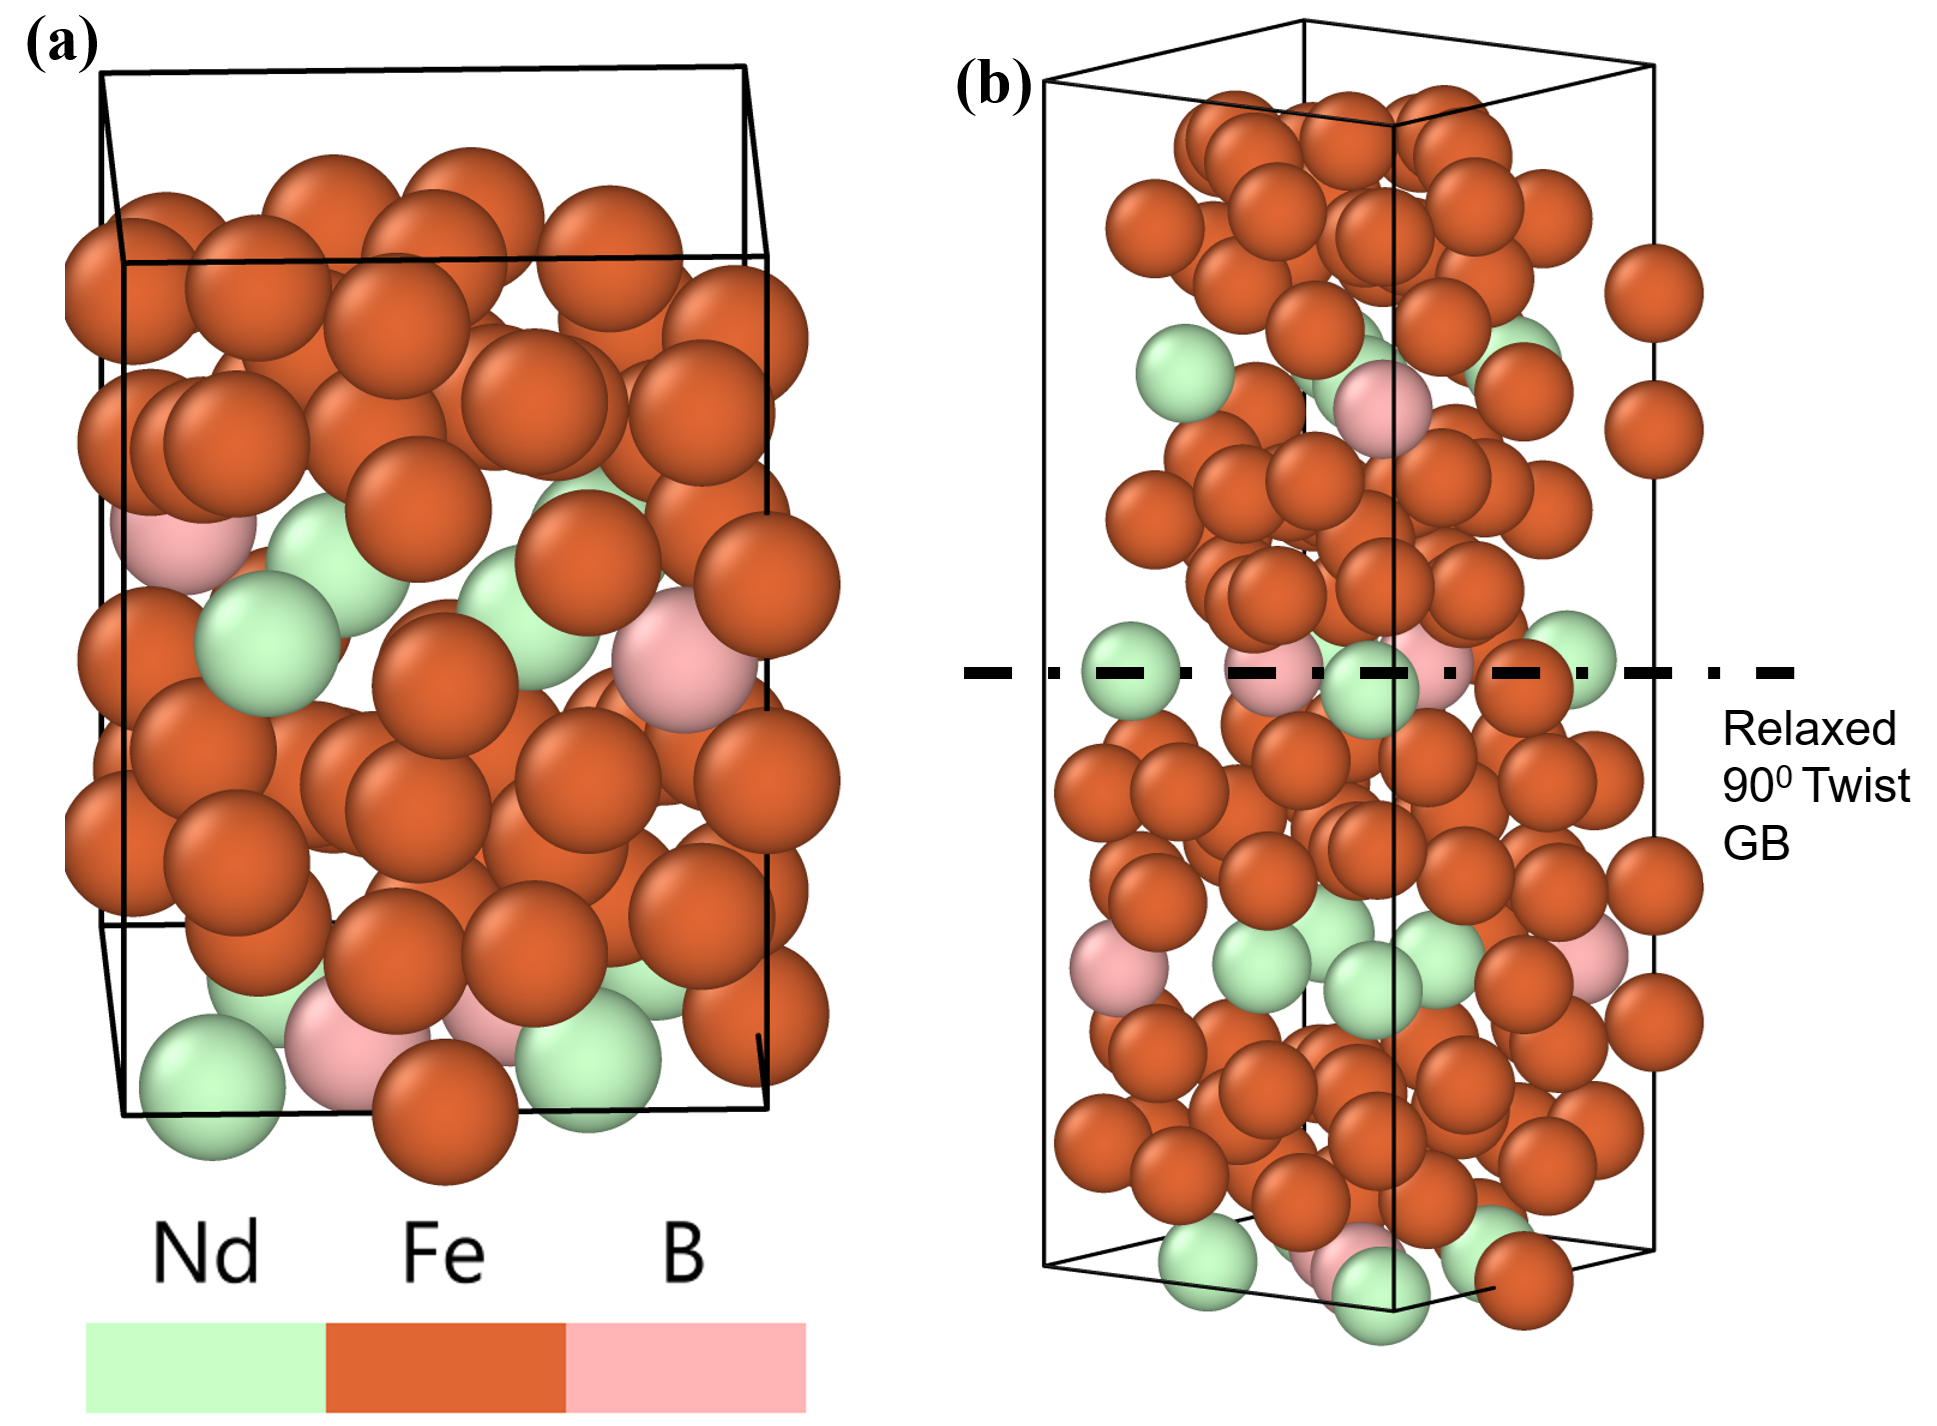
\includegraphics[width=\linewidth]{Figure_1.png}}
\caption{Structural models used in this work. (a) Relaxed bulk Nd$_2$Fe$_{14}$B supercell containing 68 atoms. \rev{(b) Relaxed 136-atom interface supercell constructed with a $90^\circ$ rotation about $[001]$, with parallel $c$ axes and a coherent rotational registry.} Rare-earth (Nd), Fe, and B atoms are shown in green, orange, and pink, respectively. The dashed line marks the grain-boundary plane.}
\rev{\label{fig:structure}}
\end{figure}

\section{Results and discussion}
\rev{The bulk calculations establish the crystal-field trends across the lanthanide series and provide a reference for assessing the grain-boundary environments. The total one-electron $4f$ ligand-field splitting decreases monotonically from 2589\invcm{} for Ce to 1002\invcm{} for Dy (Table~\ref{tab:cf}), consistent with the progressive contraction and localization of the $4f$ orbitals across the series \cite{aravena2016,freeman1962}. Gadolinium follows the same orbital-energy trend, but its half-filled $4f^7$ ground term has $L=0$ and therefore no first-order orbital anisotropy. It thus provides a useful reference for distinguishing changes in orbital splitting from changes in magnetic response. For Ce(III), the $4f^1$ configuration contains no intra-$4f$ electron pairs, and its level splittings within the present model arise from the crystal field and spin--orbit coupling. For the anisotropic ions, the dominant bulk single-ion susceptibility direction lies predominantly along the crystallographic $c$ axis in the finite-cell embedding. This behavior is qualitatively consistent with the uniaxial regime observed in $R_2$Fe$_{14}$B single crystals, although the present exchange-free calculations do not describe the low-temperature spin reorientation of magnetically ordered $\ndfeb$ \cite{hirosawa1986,yamada1988}.}

\begin{table}[H]
\centering
\caption{\rev{One-electron $4f$ orbital-energy descriptors in the finite-cell embedding: selected bulk atom~2 ($4g$) and interface atom~13 (class A, $4f$ parent).} \rev{These are distinct parent sublattices.} \rev{$\delta_{\mathrm{orb}}=\epsilon_2-\epsilon_1$ and $\Delta_{\mathrm{orb}}=\epsilon_3-\epsilon_2$ are orbital gaps, not spin--orbit doublet splittings.} \rev{Energies in cm$^{-1}$.}}
\label{tab:cf}
\small
\begin{tabular}{lccccc}
\toprule
Ion & Bulk spread & GB spread & Ratio & $\delta_{\mathrm{orb}}$ & $\Delta_{\mathrm{orb}}$ \\
 & & & & (bulk$\to$GB) & (bulk$\to$GB) \\
\midrule
Ce & \rev{2589.4} & \rev{1654.6} & \rev{0.639} & \rev{405.7$\to$5.7} & \rev{1461.0$\to$767.8} \\
Pr & \rev{1835.1} & \rev{1595.2} & \rev{0.869} & \rev{137.1$\to$4.9} & \rev{1177.0$\to$740.4} \\
Nd & \rev{1463.8} & \rev{1513.2} & \rev{1.034} & \rev{65.0$\to$4.2} & \rev{921.1$\to$703.2} \\
Gd & \rev{1064.7} & \rev{1313.6} & \rev{1.234} & \rev{18.5$\to$3.1} & \rev{478.8$\to$613.2} \\
Tb & \rev{1040.9} & \rev{1295.1} & \rev{1.244} & \rev{16.3$\to$3.1} & \rev{464.8$\to$604.7} \\
Dy & \rev{1001.6} & \rev{1261.4} & \rev{1.259} & \rev{12.0$\to$3.0} & \rev{430.9$\to$589.3} \\
\bottomrule
\end{tabular}
\end{table}

\rev{The selected-site comparison in the finite-cell model exhibits an opposite response across the lanthanide series.} The total ligand-field splitting (Fig.~\ref{fig:crossover}a) decreases substantially for the light lanthanides, falling by 36\% for Ce and 13\% for Pr, whereas it increases by 23--26\% for the heavy lanthanides Gd, Tb, and Dy. \rev{The corresponding grain-boundary-to-bulk ratio (Fig.~\ref{fig:crossover}b) crosses unity at Nd, which changes by only 3\% and therefore marks the crossover within this comparison.} \rev{Because both the parent sublattice and the finite electrostatic environment contribute, this crossover is not by itself evidence for a universal change of sign caused by the boundary.} \rev{The decrease of the bulk splitting across the series is consistent with radial contraction, but attributing the sign crossover uniquely to the radial extent of the $4f$ shell requires a radial analysis of the many-electron state beyond a representative eigenorbital.} \rev{The representative one-electron level schemes for Ce and Dy (Fig.~\ref{fig:crossover}c,d) illustrate how the finite-cell comparison drives the lowest orbital pair toward near degeneracy while modifying the next-orbital gap in opposite ways for light and heavy lanthanides.} \rev{In Dy (Fig.~\ref{fig:crossover}d), $\delta_{\mathrm{orb}}$ decreases from 12 to 3\invcm{}, while $\Delta_{\mathrm{orb}}$ increases from 431 to 589\invcm{}.} \rev{Ce exhibits the opposite change of $\Delta_{\mathrm{orb}}$ (Fig.~\ref{fig:crossover}c), from 1461 to 768\invcm{}.} \rev{These orbital separations describe the effective ligand-field operator; they are not ground-state magnetic-doublet splittings.} \rev{The many-electron first excited Kramers doublet lies at 139 and 247\invcm{} for Dy in the bulk and interface models, respectively, and at 1506 and 829\invcm{} for Ce (Supplementary Table~S4).} \rev{Thus Dy's magnetic ground doublet is more isolated in this particular comparison, while Ce's first doublet excitation decreases.} \rev{This single-ion response is relevant to anisotropy, but cannot alone explain the coercivity obtained by grain-boundary diffusion \cite{hono2012,sepehriamin2013,patrick2024}.}

\begin{figure}[H]
\rev{\centering}
\rev{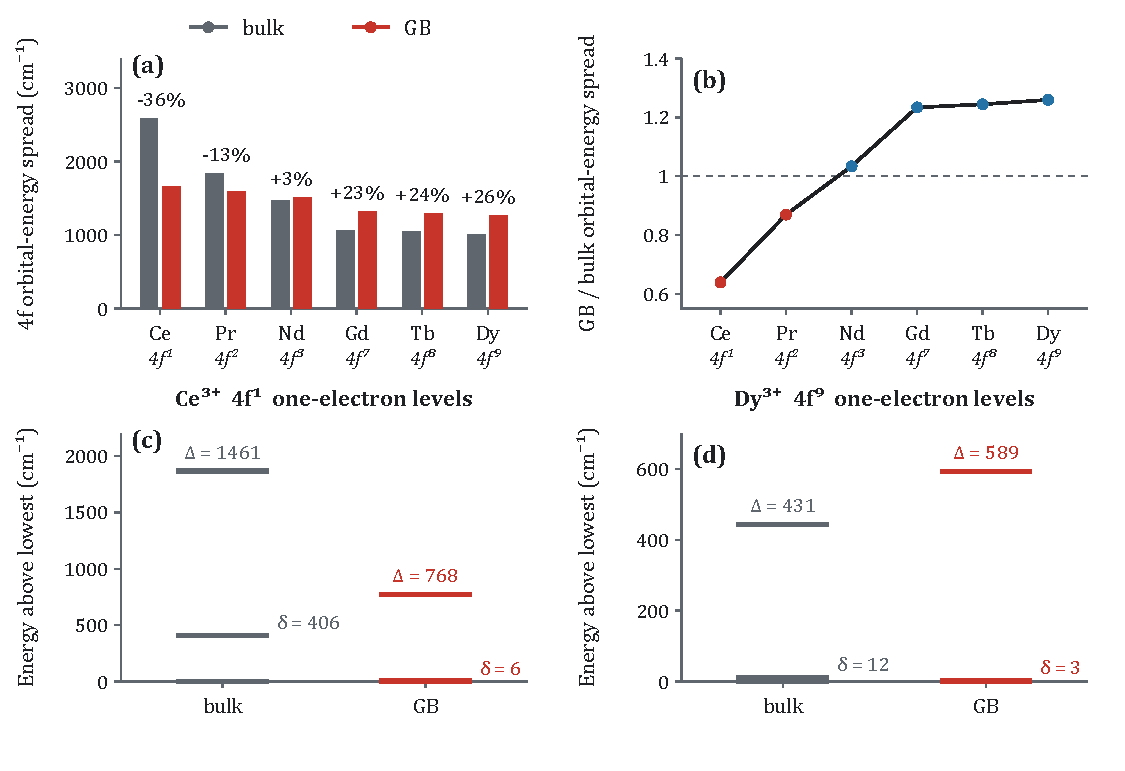
\includegraphics[width=\linewidth]{Figure_2.pdf}}
\caption{\rev{Finite-cell comparison of the selected bulk and interface sites.} \rev{(a) Total one-electron $4f$ orbital-energy spread.} \rev{(b) Ratio of GB-to-bulk spread.} \rev{Lowest one-electron AILFT orbital levels for (c) Ce$^{3+}$ and (d) Dy$^{3+}$; $\delta$ denotes $\delta_{\mathrm{orb}}$ and $\Delta$ denotes $\Delta_{\mathrm{orb}}$ of Table~\ref{tab:cf}.} \rev{Magnetic multiplet energies are given separately in Supplementary Table~S4.}}
\rev{\label{fig:crossover}}
\end{figure}

\rev{A rank decomposition makes the light--heavy contrast more quantitative without assuming a radial mechanism.} \rev{In the finite-cell comparison, the rank-2 strength $S_2$ changes by $-27\%$ (Ce), $-8\%$ (Pr), $+7\%$ (Nd), and $+26$--$28\%$ (Gd, Tb, Dy), while $S_4$ and $S_6$ decrease throughout the series (Supplementary Fig.~S2a and Table~S5).} \rev{The competition between these components explains why the total orbital-energy spread does not follow one rank alone.} \rev{The decomposition is exact for the extracted one-electron AILFT matrix.} \rev{It separates angular ranks, rather than assigning additive contributions to individual ligand shells or measuring radial contraction.} \rev{The modified crystal field also changes the orientation of the local magnetic response in the finite-cell model.} \rev{The schematic in Fig.~\ref{fig:chit}a illustrates the rotation from the predominantly bulk $c$ direction toward the basal plane at the interface.} \rev{Fig.~\ref{fig:chit}b uses a consistent definition for all six ions: the angle between the principal axes of the largest zero-field susceptibility eigenvalue at 2~K.} \rev{Bulk and interface records are selected by their explicit run labels; auxiliary calculations are excluded from this comparison (Supplementary Sec.~S2).} \rev{The values obtained directly from the saved susceptibility tensors are 87.0$^\circ$ (Ce), 87.4$^\circ$ (Pr), 87.6$^\circ$ (Nd), 87.1$^\circ$ (Gd), 87.3$^\circ$ (Tb), and 87.4$^\circ$ (Dy).} \rev{The Gd value represents the principal-axis rotation of the calculated single-ion susceptibility tensor, rather than an assignment of first-order orbital anisotropy.} \rev{These single-ion directions describe the chosen finite embedding and are not the equilibrium magnetization directions in the exchange-coupled host.} \rev{A misoriented local response can affect reversal, but its angle alone does not establish preferential reverse-domain nucleation.}

\begin{figure}[H]
\rev{\centering}
\rev{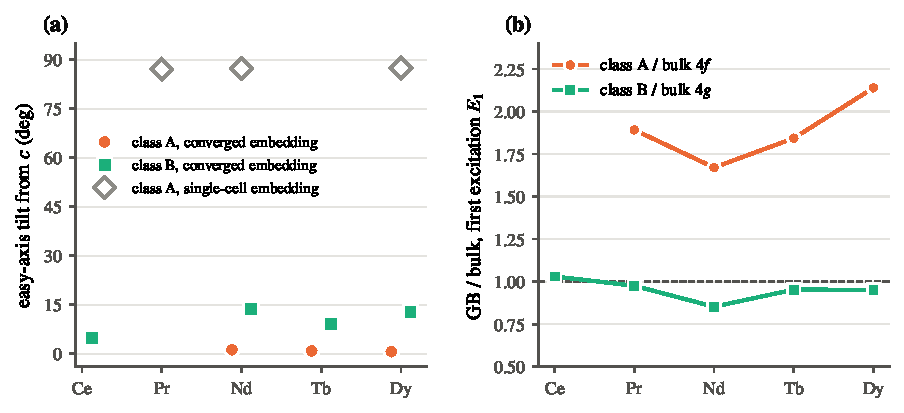
\includegraphics[width=\linewidth]{Figure_3.pdf}}
\caption{\rev{Local magnetic response in the finite-cell embedding.} \rev{(a) Schematic rotation of the dominant single-ion susceptibility direction from bulk toward the interface basal plane.} \rev{(b) Angle between the bulk and interface zero-field susceptibility principal axes at 2~K, evaluated from the calculated tensors.} \rev{The Gd value represents the principal-axis rotation of the calculated single-ion susceptibility tensor, rather than an assignment of first-order orbital anisotropy.} \rev{No Fe exchange field is included.}}
\rev{\label{fig:chit}}
\end{figure}

\rev{For scale, a Stoner--Wohlfarth uniaxial coherent-rotation model gives $H_{\mathrm{sw}}/H_A=(|\cos\theta|^{2/3}+|\sin\theta|^{2/3})^{-3/2}$, where $H_A=2K/(\mu_0M_s)$ and $\theta$ is the angle between the easy direction and the applied field \cite{stoner1948}.} \rev{Taking the applied field along the bulk response axis, the 87.0--87.6$^\circ$ interface angles yield $H_{\mathrm{sw}}/H_A\simeq0.82$--$0.85$ (Supplementary Table~S9).} \rev{This is an illustrative loss-of-metastability field for an isolated uniaxial region, not a calculated nucleation field or hysteretic coercivity of the magnet.} \rev{It assumes a known $K$ and omits exchange with the grain interior, demagnetizing fields, intergranular phases, and nonuniform reversal.} \rev{In particular, the orbital-energy spread cannot be substituted for $K$.} \rev{The calculation therefore identifies a possible single-ion contribution rather than proving a nucleation site.}

\rev{The calculated single-ion susceptibility illustrates the magnetic consequences of the same finite-cell Hamiltonians (Fig.~\ref{fig:easyaxis}).} The largest differences between bulk and grain-boundary environments occur at low temperature, where only the lowest crystal-field levels contribute to the magnetic response. \rev{Pr provides the clearest example (Fig.~\ref{fig:easyaxis}b): the bulk $\overline{\chi}_M T$ is strongly reduced at low temperature, whereas the interface value remains larger over the plotted range.} \rev{A decrease of $\chi T$ is not by itself evidence that $\chi$ vanishes or that a different magnetic ground-state multiplicity has been established; a singlet can retain a Van Vleck susceptibility.} \rev{Dy (Fig.~\ref{fig:easyaxis}f) exhibits a modestly enhanced low-temperature response, while Tb changes only slightly.} \rev{Gadolinium (Fig.~\ref{fig:easyaxis}d) remains nearly unchanged between the environments in its orientational mean, consistent with its $S$-state character.} \rev{These curves are useful descriptors of the isolated-ion models.} \rev{Comparison with SQUID measurements of ferromagnetic $\ndfeb$ would require the Fe exchange field and the collective magnetic response, so direct experimental validation cannot be inferred from Fig.~\ref{fig:easyaxis} alone.}

\begin{figure}[H]
\rev{\centering}
\rev{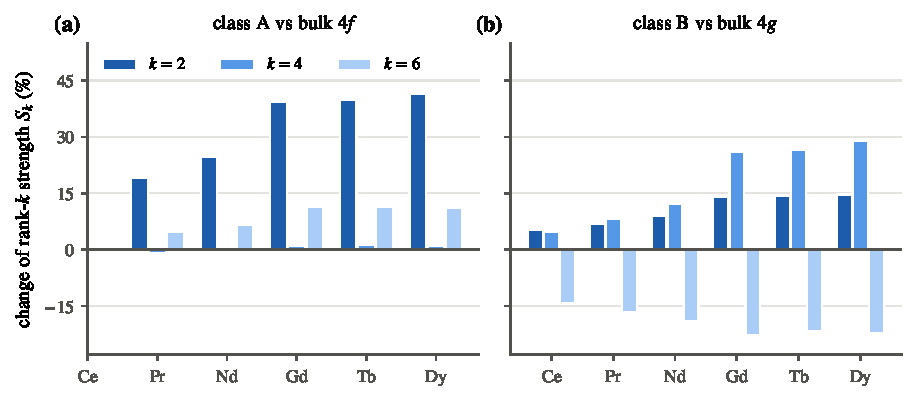
\includegraphics[width=\linewidth]{Figure_4.pdf}}
\caption{\rev{Calculated temperature dependence of the orientational mean $\overline{\chi}_M T$ for (a) Ce$^{3+}$, (b) Pr$^{3+}$, (c) Nd$^{3+}$, (d) Gd$^{3+}$, (e) Tb$^{3+}$, and (f) Dy$^{3+}$ in the finite-cell bulk and interface environments.} \rev{Dashed lines denote the corresponding free-ion Curie constants.} \rev{These zero-field single-ion calculations omit the Fe exchange field.}}
\rev{\label{fig:easyaxis}}
\end{figure}

\rev{The real-space form of a representative AILFT $4f$ orbital is illustrated in Fig.~\ref{fig:orbital}. The selected bulk environments of Ce, Pr, and Dy are shown in Fig.~\ref{fig:orbital}(a--c), respectively, and the corresponding interface environments are shown in Fig.~\ref{fig:orbital}(d--f), using the archived orbital-27 cube files. The titles identify the ion, Bulk or GB environment, and archived orbital index MO27. The full one-electron density is projected along $c$ onto the $a,b$ plane, and all six distributions share a density range of 0--7~\AA$^{-2}$. A common square-root color mapping makes weak lobes visible while retaining physical density values on the colorbar \cite{crameri2020}. This mapping changes only the display, not the density integrals or orbital radii. The bulk--interface comparison reveals changes in spatial distribution that are not apparent from the interface distributions alone. The root-mean-square radius of this eigenorbital decreases from 0.84 to 0.61~\AA{} for Ce, from 0.66 to 0.58~\AA{} for Pr, and from 0.47 to 0.46~\AA{} for Dy (Supplementary Table~S10). The selected orbital therefore becomes more compact at the interface in all three cases; these results do not support an expansion of the light-ion orbital there. These quantities characterize individual eigenorbitals rather than the total correlated $4f$ density, and nearly degenerate orbitals can mix. The distributions illustrate the stated finite-cell model and different parent sites without establishing a unique radial origin of the sign crossover or determining the magnetic easy direction. The environment-resolved one-electron Hamiltonians provide parameters for effective spin models, provided that spin--orbit coupling, exchange, and model validation are treated consistently \cite{tranchida2018,nitol2026,corvacho2026,murillopolo2026,eriksson2017}.}

\begin{figure}[H]
\centering
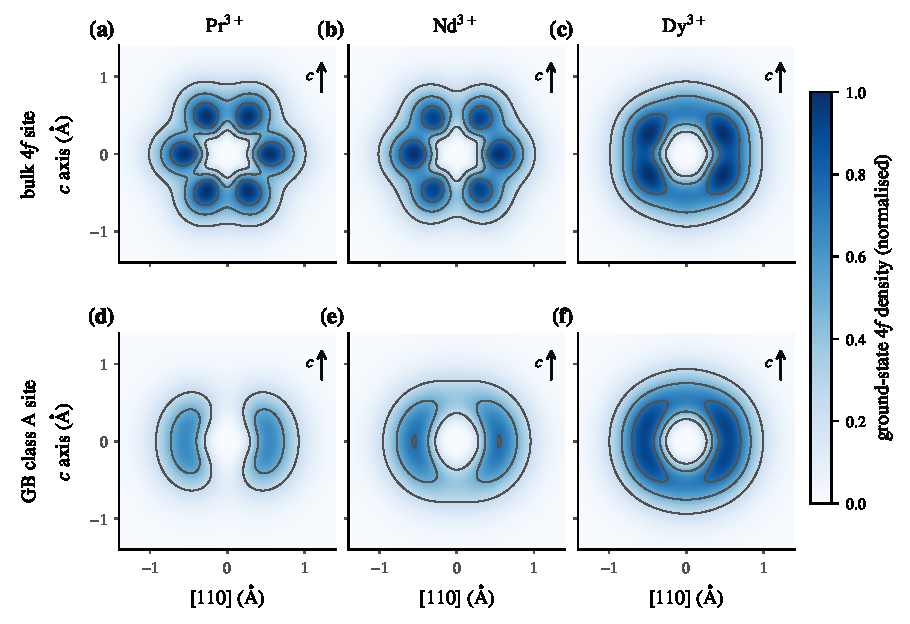
\includegraphics[width=\linewidth]{Figure_5.pdf}
\caption{\rev{Projected density of the lowest AILFT one-electron $4f$ orbital (MO27, orbital~27 in the archived files) for Ce (a,d), Pr (b,e), and Dy (c,f). The selected bulk atom~2 is shown in (a--c), and interface atom~13 is shown in (d--f), using the finite-cell embedding. The titles identify the ion and environment (Bulk or GB). Both spatial axes have labeled 0.5~\AA{} intervals and minor ticks every 0.25~\AA. Thin black contours indicate projected densities of 0.25, 0.75, and 2.0~\AA$^{-2}$, with identical contour levels throughout. The full orbital density is integrated along $c$ and projected onto the $a,b$ plane, centered on the rare-earth ion. All six distributions use the same 0--7~\AA$^{-2}$ density range and square-root color mapping ($\gamma=1/2$); colorbar ticks give the physical projected density. Each three-dimensional orbital is normalized to one electron. The annotated $r_{\mathrm{rms}}$ is calculated from the full three-dimensional cube. These distributions represent individual orbital densities rather than crystal-field potentials or total $4f$ densities; the bulk and interface sites have different parent sublattices.}}
\label{fig:orbital}
\end{figure}

\rev{We tested the electrostatic embedding to determine how the surrounding charge distribution affects the calculated crystal fields. Supplementary Fig.~S1(a,b) and Table~S6 compare the finite-cell results with ion-centered spherical embeddings of 18 and 25~\AA{} radius. The spherical embeddings use rare-earth $+3$, B $-3$, and Fe $-3/14$ charges, with the residual charge distributed over the outermost 2~\AA{} shell. This changes both the charge assignment and the size and shape of the environment relative to the finite-cell model. Therefore, the finite-cell and sphere calculations test the combined effects of these changes. Comparing the two sphere radii separately tests the radius dependence within the same charge convention. At the Nd interface site, $\Atwo$ changes from $-933$ to $+784$\invcm{}, and the large rotation toward the basal plane is absent in the sphere model. Increasing the sphere radius from 18 to 25~\AA{} changes the tested-site axial parameters by approximately 5--8\% and the interface-atom-13-to-bulk-atom-2 ratio by 13--14\%. Changing the charge partition produces changes of 33--78\% in the axial parameters, while SC-NEVPT2 produces changes of approximately 11--18\% in the tested sphere calculations. These values describe the sensitivity of the tested sites and should not be used as general uncertainty bounds. The results show that the magnitude and sign of the local crystal-field response depend on the embedding. Charge neutrality alone does not establish the accuracy of the local electrostatic potential.} \rev{We also compared interface and bulk sites belonging to the same parent sublattice. In the 25~\AA{} sphere model, the class A axial parameter increases by 30--58\% relative to the bulk $4f$ site, whereas class B changes by at most approximately 4\% relative to the bulk $4g$ site (Supplementary Fig.~S1(c,d) and Table~S7). The total orbital splitting increases at both site classes in the converged calculations. The sign crossover shown in Fig.~\ref{fig:crossover} is therefore not retained in these comparisons. For Nd and Dy, the calculated bulk ordering $\Atwo(4g)>\Atwo(4f)$ agrees with site-resolved DFT results. Magnetization analyses also distinguish the crystal-field environments of the two sublattices \cite{tatetsu2018,boust2022,cadogan1988}. For Ce, stable seven-$f$-orbital SA-CASSCF solutions were not obtained at the two $4f$-parent sites, and these entries are excluded from the sphere-model comparison. The available ground-doublet $g$-tensor axes for Ce, Nd, and Dy remain within 14$^\circ$ of the crystallographic $c$ axis at the unmodified interface. Adding capped effective core potentials to neighboring atoms changes the matched interface-to-bulk axial-parameter ratios by less than 0.5\% at the tested level (Supplementary Table~S8). These calculations test short-range core repulsion, but do not include explicit Fe--$4f$ covalency or metallic screening. Thus, the crossover and large reorientation obtained in the finite-cell model depend on the selected sites and electrostatic embedding. They cannot be assigned to grain-boundary geometry alone.}

\rev{The present structural model contains two inequivalent boundary-plane sites, classes A and B, in one coherent rotational-registry interface. Other boundary structures need to be studied before extending these results to sintered magnets. General tilt and twist boundaries, different interfacial translations, and Nd/Pr-rich wetting phases can change the local symmetry and exchange coupling. Residual Cu, Co, Zr, B, and oxygen can also change the coordination, electrostatics, and magnetic connectivity. These effects are not included in the six trivalent-ion substitutions studied here. Ce$^{3+}$ was treated as a fixed-$4f^1$ reference to allow a common comparison across the lanthanide series. Determining the equilibrium Ce valence requires a model that includes Ce$^{4+}$ and possible mixed-valence behavior \cite{capehart1993,alam2013}. The active-space instability found in some Ce calculations does not establish a valence transition.} \rev{The present approach complements density-functional calculations of local crystal-field perturbations. Patrick et al.\ studied Ti-induced perturbations in SmFe$_{12}$ \cite{patrick2024}. Both approaches determine how the local environment changes the crystal-field operator, including its lower-symmetry components. The multireference calculations used here also resolve the localized many-electron multiplets and their exchange-free magnetic response across the lanthanide series. A quantitative comparison between the unscreened point-charge fields and screened density-functional fields requires further validation. In experiments, grain-boundary diffusion changes anisotropy, exchange, segregation, and intergranular structure \cite{hono2012,sepehriamin2013,sepehriamin2023}. Our calculations address the single-ion electronic contribution to these changes. Conventional sintered magnets have coercivities of order $0.2H_A$ \cite{hono2012}, while two-step Dy grain-boundary diffusion in fine-grained, initially Dy-free sintered magnets has achieved $\mu_0H_c=2.8$~T \cite{sepehriamin2023}. The isolated-region switching estimate shows how local-axis orientation can affect switching under the stated assumptions. Predicting the measured coercivity also requires exchange coupling, demagnetizing fields, and collective magnetization reversal.}


\section{Conclusions}

\rev{The local $4f$ electronic structure in bulk and grain-boundary environments of $\ndfeb$ was investigated using embedded multireference calculations with spin--orbit coupling. The calculations were performed for Ce, Pr, Nd, Gd, Tb, and Dy to determine the crystal-field parameters, orbital energies, magnetic multiplets, and temperature-dependent single-ion susceptibilities. In the finite-cell comparison, the total orbital splitting decreases by 36\% for Ce and 13\% for Pr, increases by 23--26\% for Gd, Tb, and Dy, and changes by only 3\% for Nd. The dominant low-temperature susceptibility axes rotate from the bulk $c$ direction toward the basal plane.} \rev{This work extends the multireference framework used in molecular magnetism to rare-earth sites in an intermetallic permanent magnet. By resolving the local Hamiltonian across different environments and substitutions, we directly connect atomic coordination with the electronic states responsible for the single-ion magnetic response. This approach provides a link between the microstructural descriptions used in physical and powder metallurgy and the quantum chemical description of localized $4f$ electrons. The matched-site calculations also show that inequivalent interface sites can respond differently, highlighting the importance of resolving individual rare-earth environments.} \rev{The calculated responses depend on the electrostatic embedding and site selection. Future work will incorporate metallic screening and Fe exchange and examine a broader range of matched bulk and grain-boundary sites to assess the robustness of these trends. The present calculations provide environment-resolved single-ion Hamiltonians and a systematic framework for studying how local chemistry and microstructure modify rare-earth magnetism. These quantities form the microscopic electronic inputs needed to connect quantum chemical calculations with multiscale models of permanent magnets.}

\section*{Data availability}
\rev{The relaxed bulk and interface structures, selected crystal-field tables, and complete complex Wybourne parameters for the archived calculations accompany the supplementary material.} \rev{The underlying input files, raw output files, and orbital cubes are available from the authors on reasonable request.}

\section*{Acknowledgements}
This work was supported by the Department of Mechanical and Electrical Engineering at Merrimack College. The author acknowledges the use of computational resources at the Massachusetts Green High Performance Computing Center (MGHPCC). This research also benefited from high performance computing allocations provided by the National Science Foundation through ACCESS (awards MAT250103 and MAT240094). Additional computational resources were supported by Argonne National Laboratory under the Director's Discretionary allocation for the project \textit{AIAlloyLW}. Further support was provided through a National Science Foundation MRI Award to Wilkes University (Award No.\ 1920129), which contributed essential computational infrastructure for this study.

\bibliographystyle{elsarticle-num}
\bibliography{references}

\end{document}